\chapter{基于功率消耗和鲁棒自适应博弈控制的负载分配策略}
在协同吊挂系统中,如果一个直升机在飞行过程中提前耗尽能量或失效,协同运输会直接崩溃。可见,在综合考虑各直升机相对位置、性能差异的前提下,合理分配吊挂负载给各个直升机,具有重要意义。为此,本文提出了基于功率消耗和鲁棒自适应博弈控制的负载分配策略。第\ref{section:chap_4_introduction}节首先以四个纵列式直升机协同吊挂系统为研究对象,基于以吊挂物为主导的分层控制策略,将负载分配问题分解为期望吊索拉力计算和抗干扰吊索拉力计算两部分。第\ref{section:power_distribution}节训练得到了直升机神经网络功率代理模型,提出了基于功率消耗的负载分配策略。第\ref{section:game_distribution}节考虑直升机性能差异、互动影响,提出了基于鲁棒自适应微分博弈控制的抗干扰负载分配策略。最后,仿真对比了基于功率消耗、绳索拉力的负载分配策略的优缺点;验证了各直升机性能存在差异时期望吊索拉力优化计算方法的可行性;针对不同值函数验证了博弈控制的可行性和鲁棒性;分析了基于整个分配策略的仿真结果。

\section{引言}\label{section:chap_4_introduction}
在直升机协同吊挂系统中,如果其中一架或几架直升机提前耗尽能量或发生故障,且吊挂物重量大于剩余直升机的负载能力时,整个协同吊挂系统将会失效,甚至发生吊索交叉、直升机相互碰撞等高危情况。所以,合理分配负载给各个直升机,使各个直升机在协同运输过程中功耗相等、航时航程一致,是必要的。

\begin{figure}[!htb]  
  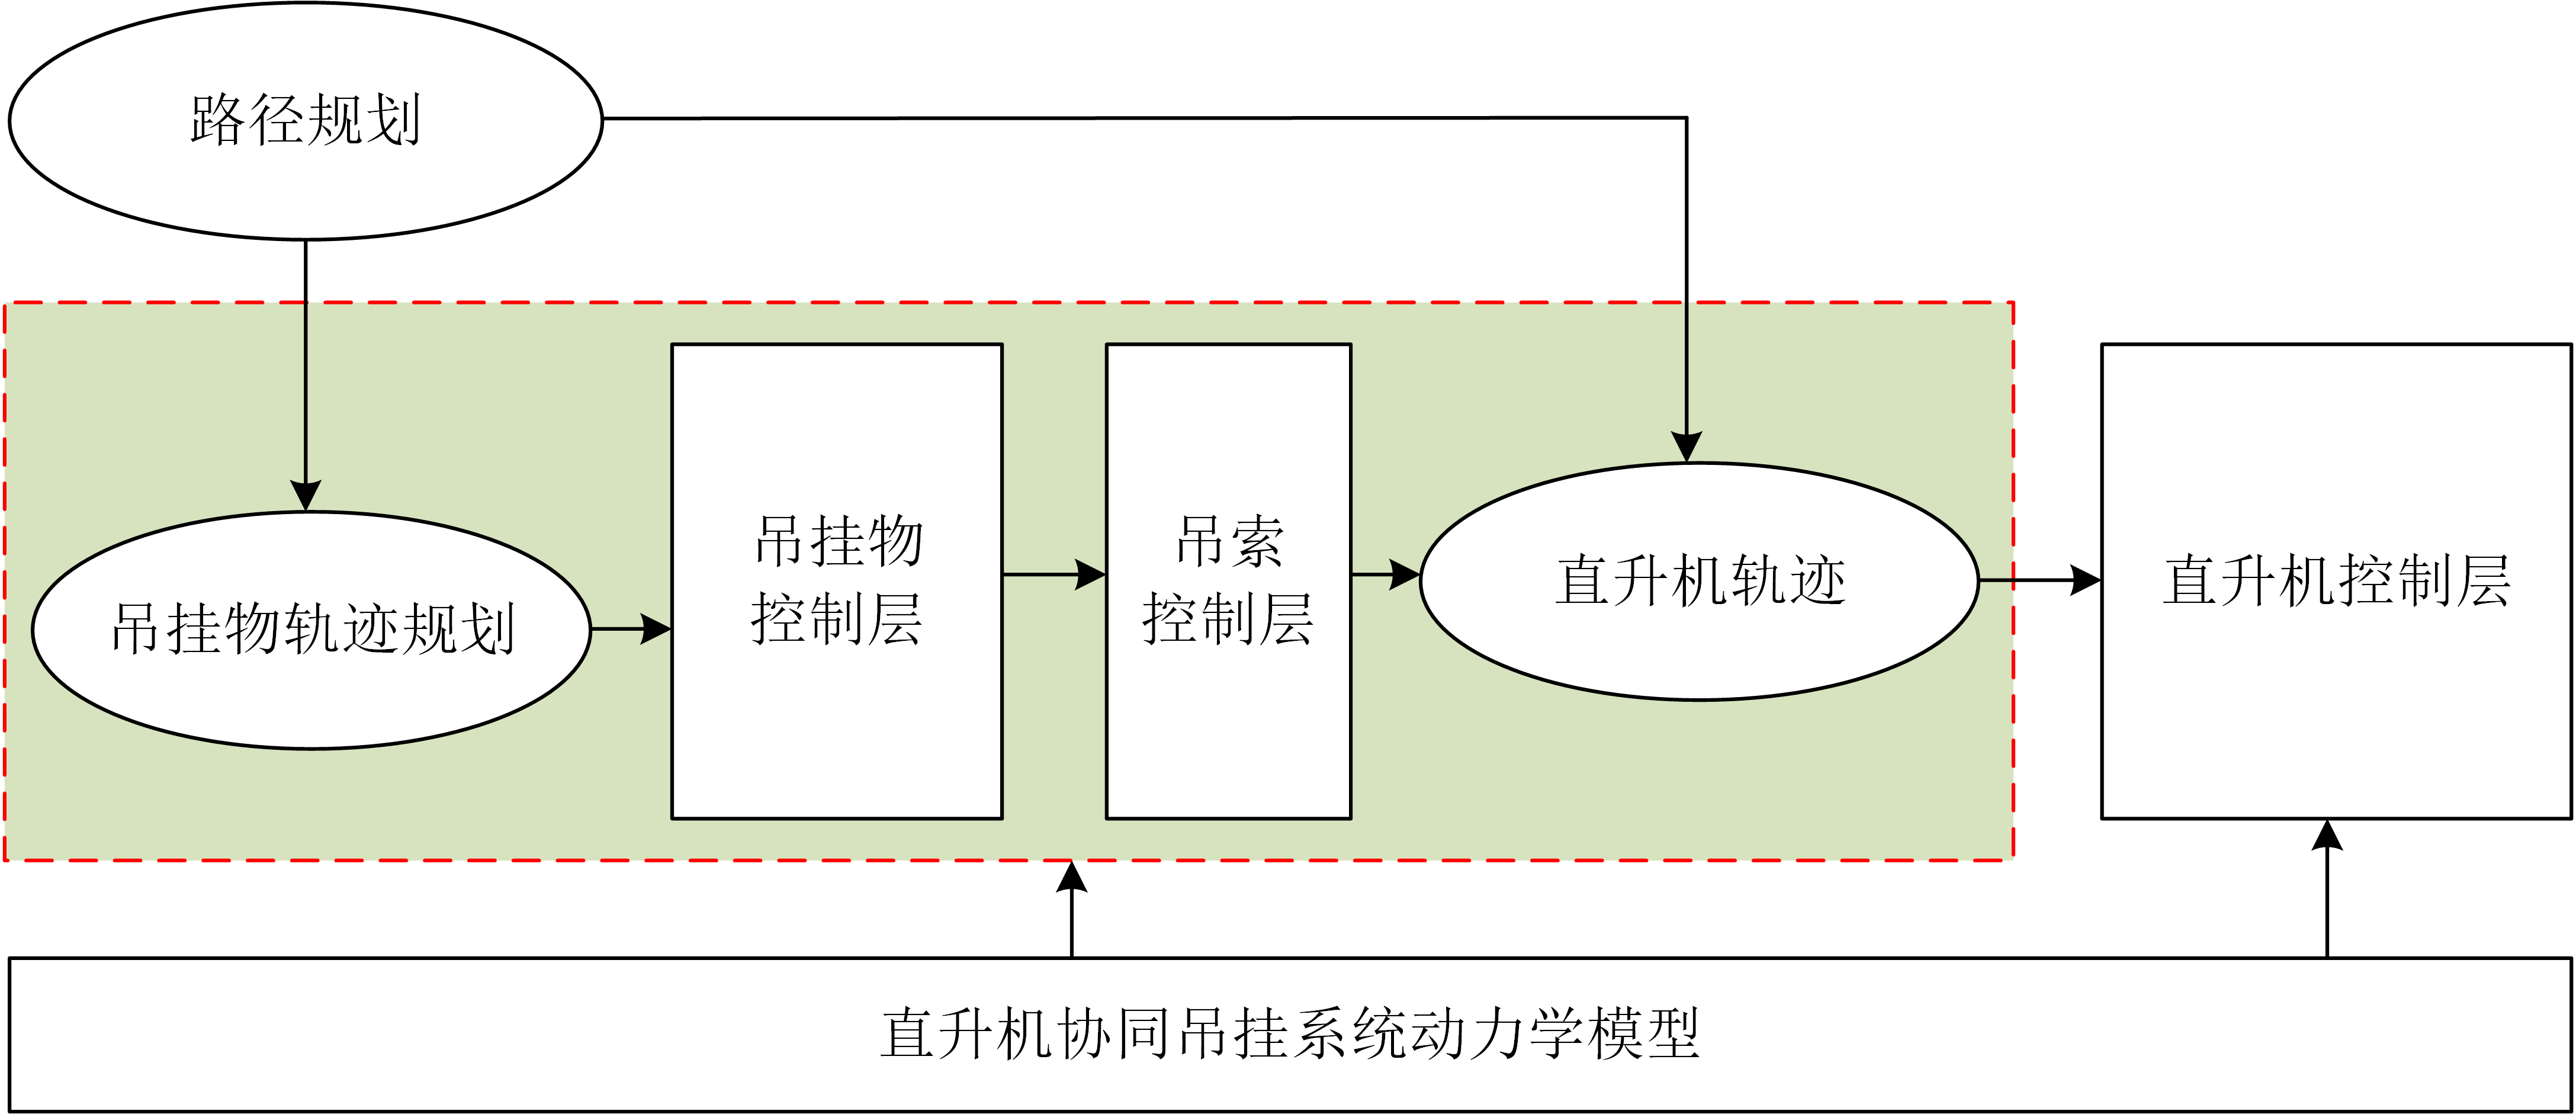
\includegraphics[width=10cm]{fig/figure_chap4/Chap4_1_1.png}
  \caption{直升机协同吊挂系统分层控制技术}
  \label{fig:4_1_1}
\end{figure}

以吊挂物为主导的直升机协同吊挂系统分层控制技术(见图\ref{fig:4_1_1})主要包括以下三个方面:
\begin{enumerate}
  \item 吊挂物层:根据吊挂物期望轨迹和状态,计算需要吊索提供的期望合力、合力矩。同时考虑到外界环境干扰等,设计跟随控制控制律,计算需要吊索额外提供的抗干扰合力、合力矩。将两者相加,得到需要吊索提供的全部合力、合力矩。
  \item 吊索层:根据需要吊索提供的合力、合力矩,计算需要每根吊索提供的力。在某一特定飞行状态下,吊索拉力和方向直接影响各个直升机的功率消耗。
  \item 直升机层:根据需要每根吊索提供的力,计算各个直升机的期望位置。合理设计控制策略,跟随期望位置。
\end{enumerate}

假设路径已知,基于以吊挂物为主导的直升机协同吊挂系统分层控制技术,负载分配策略可以分为期望吊索力和抗干扰吊索力计算两部分。为此,考虑各个直升机性能、位置、状态、约束差异等,本文提出了基于功率消耗的稳态负载分配策略和基于鲁棒自适应博弈跟随控制的抗干扰分配策略。

\section{基于功率消耗的期望负载分配策略}\label{section:power_distribution}
以往多数文献大多采用基于吊索拉力相等的期望负载分配策略。但随着协同吊挂系统前飞速度的增加,吊索拉力相等并不能保证各个直升机功率消耗相等。可见,这种分配策略策略仅适用于悬停、小速度飞行或机动较小的情况。因此,提出基于功率消耗的期望负载分配策略,保证在整个飞行包线内各直升机功耗相等,是有重要意义的。
\subsection{功率代理模型}
直升机功率是在配平基础上计算得到的。各个直升机动力学模型中有30个状态量,配平本身就很困难。同时考虑到基于功率消耗的期望负载分配策略要用优化方法来解决,若每次迭代均在线配平计算功率消耗,复杂度高、计算时间长。为此,提出了基于BP神经网络的功率代理模型。
\subsubsection{功率计算与分析}
假设每个纵列式直升机的吊挂点均位于重心处。则对直升机$i$,在其体轴系$x_{ib}y_{ib}z_{ib}$下,吊索作用在直升机重心的吊索力和力矩为
\begin{equation}
  {{\mathbf{M}}_{cable,i}} = \left[ {\begin{array}{*{20}{c}}
    {^i{{\mathbf{R}}_e}{\;^e}{{\mathbf{R}}_L}{\;^L}{{\mathbf{f}}_{cable.i}}} \\ 
    {{{\mathbf{0}}_{3 \times 1}}} 
  \end{array}} \right]
\end{equation}
其中,${\;^i}{{\bf{R}}_e}$为轴系$x_{e}y_{e}z_{e}$到$x_{ib}y_{ib}z_{ib}$的转换矩阵。

\begin{figure}[!htb]
  \subfloat[悬停]{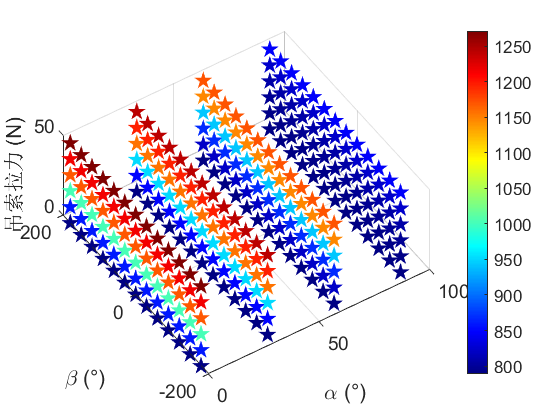
\includegraphics[width=7cm]{fig/figure_chap4/Chap4_2_1.png}}\quad
  \subfloat[前进比0.1]{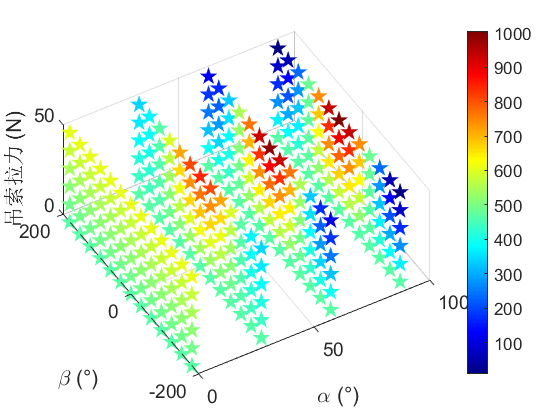
\includegraphics[width=7cm]{fig/figure_chap4/Chap4_2_2.png}}
  \caption{功率消耗计算结果}
  \label{fig:4_2_1}
\end{figure}

在吊索力作用下,采用牛顿法配平各个直升机,进而根据配平得到的状态量和操纵量计算得到功率。以悬停和前进比0.1时的功率消耗为例,见图\ref{fig:4_2_1},可以看出,悬停时功率消耗主要与吊索拉力有关。这是以往文献中较多采用基于吊索拉力均等的负载分配策略的原因。

然而,前进比为0.1时,除吊索拉力外,角$\beta$也是重要影响因素。在“2-lead”协同吊挂系统中,前面两侧直升机(直升机3、4)角$\beta$处于-90\degree 到90\degree 之间,吊索拉力作用等同于对直升机施加向后的阻力,功率消耗大。后方直升机(直升机1、2)角$\beta$处于-180\degree 到-90\degree、90\degree 到180\degree 之间,吊索拉力作用等同于对直升机施加向前的拉力,功率消耗小。可见,有一定的前飞速度时,即使吊索拉力相同,前方直升机的功率依旧会大于后方直升机。这与参考文献\cite{enciu2017flight,song2013modeling}中的计算结果吻合。

此外,需要指出的是,直升机协同吊挂系统是典型的近距离编队飞行。直升机之间不仅存在复杂的动力学耦合关系,而且存在严重的气动干扰。根据之前的计算结果\cite{Duan2021Underreview}可知,前飞时的气动干扰最大,且由气动干扰引起的功率变化比较复杂、难以建模。此外,研究发现当纵列式直升机间的距离大于小2.5倍的旋翼直径时,针对本文研究的四纵列式直升机协同吊挂系统,气动干扰可以忽略不计。因此,本文没有将气动干扰引起的功率变化引入到代理模型中,而是将下文优化过程中直升机间的安全距离约束设置为了2.5倍的旋翼直径。
\subsubsection{基于神经网络的代理模型}
BP神经网络是典型多层前向网络,如图\ref{fig:4_2_2}所示,主要由信号正向传播和误差反向传播组成。正向传播指信号依次经过输入、隐层神经元,再由输出神经元输出的过程。反向传播是指,当输出值与目标值之间存在误差时,将误差反向传播,并由梯度下降算法更新网络权值、阈值的过程。当误差足够小时,网络反向传播停止,BP神经网络训练完成。
\begin{figure}[!htb]
  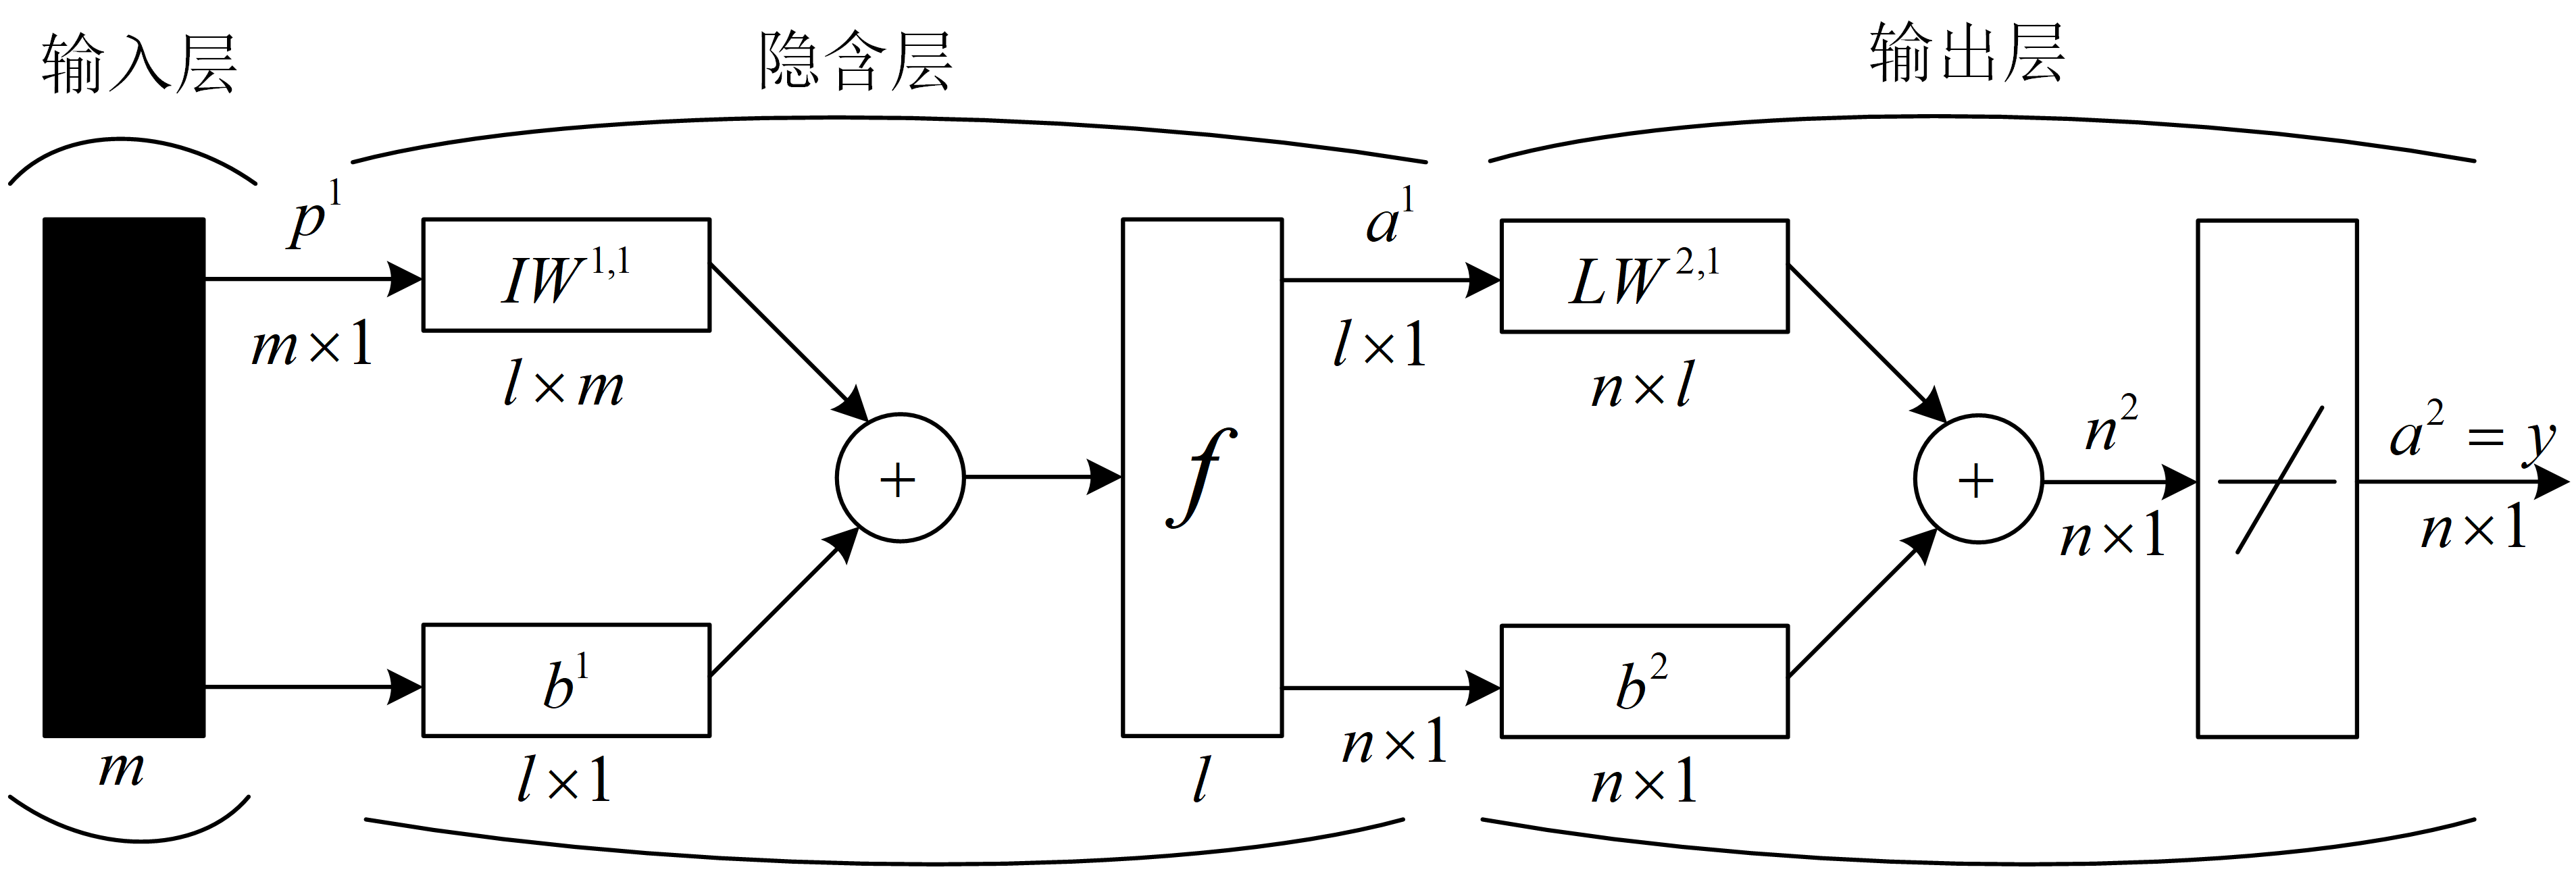
\includegraphics[width=8cm]{fig/figure_chap4/Chap4_2_3.png}
  \caption{BP神经网络}
  \label{fig:4_2_2}
\end{figure}

针对纵列式直升机神经网络功率代理模型,输入层有4个变量:前进比、角$\alpha$、角$\beta$、吊索拉力。根据问题复杂度,隐含层设计了40个神经元。神经网络输出为直升机的功率消耗。此外,隐含层的激活函数为双曲正切函数,输出层的激活函数为恒等映射函数。

用于训练功率代理模型的数据集前进比取值为0到0.11,角$\alpha$取值为0到$\frac{\pi}{2}$,角$\beta$取值为$-\pi$到$\pi$,吊索拉力取值为0到100 N(吊挂物重量)。经过上述过程,共得到4680个数据点,其中4000个数据点用来训练神经网络,剩余的680个数据点用来验证神经网络的有效性。从图\ref{fig:4_2_3}可以看出,真实值与神经网络输出值拟合很好。这表明训练得到的功率代理模型是有效的,可以在下文的优化工作中使用。
\begin{figure}[!htb]
  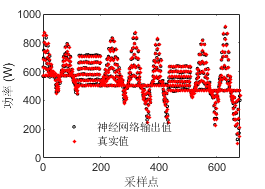
\includegraphics[width=7cm]{fig/figure_chap4/Chap4_2_4.png}
  \caption{基于BP神经网络的功率消耗拟合结果}
  \label{fig:4_2_3}
\end{figure}

\subsection{负载分配优化模型}
\subsubsection{设计变量}
针对4个纵列式直升机协同运输一个吊挂物的系统,选择4根吊索的力矢量作为设计变量,如下
\begin{equation}
  {\bf{u}} = \left[ {^L{f_{cable,1x}},{\;^L}{f_{cable,1y}},{\;^L}{f_{cable,1z}},\; \cdots ,{\;^L}{f_{cable,4x}},{\;^L}{f_{cable,4y}},{\;^L}{f_{cable,4z}}} \right]^T
\end{equation}
\subsubsection{约束}
首先,吊索力矢量需满足吊挂物的动力学方程,见式\ref{equation:chap_4_1}。将吊索作用力$\bf{M}_c$移到左侧,式\ref{equation:chap_4_1}也可以写作
\begin{equation}
  \left[ {\begin{array}{*{20}{c}}
    {{{\bf{I}}_{3 \times 3}}}&{{{\bf{I}}_{3 \times 3}}}&{{{\bf{I}}_{3 \times 3}}}&{{{\bf{I}}_{3 \times 3}}}\\
    {{{\left( {{{\bf{h}}_1}} \right)}^*}}&{{{\left( {{{\bf{h}}_2}} \right)}^*}}&{{{\left( {{{\bf{h}}_3}} \right)}^*}}&{{{\left( {{{\bf{h}}_4}} \right)}^*}}
    \end{array}} \right]{\bf{u}} = {{\bf{M}}_L}{\bf{\ddot x}} + {{\bf{C}}_L}{\bf{\dot x}} - {{\bf{g}}_L} - {{\bf{M}}_{aero}}
    \label{equation:chap_4_8}
\end{equation}
其中,${{{\left( {{{\bf{h}}_i}} \right)}^*}}$是向量${{{\bf{h}}_i}}$的斜对称矩阵。

为了避免直升机间相互碰撞、减少气动干扰,引入直升机间的安全距离约束如下
\begin{equation}
  \left\| {^e{{\bf{P}}_i} - {\;^e}{{\bf{P}}_j}} \right\| \ge {d_{\min }}\;\;\;\;\;\;\;\;\;i,j = 1,2,3,4
\end{equation}
其中,$d_{\min}$等于4.5 m(2.5倍的旋翼直径)。事实上,直升机间的距离越大,角$\alpha$越大,负载相同的吊挂物需要的吊索拉力越大。吊索拉力越大,直升机功率消耗也越大,这对优化目标是不利的。使用长吊索可以缓解这种不利情况,经过计算发现本文研究的四纵列式直升机协同吊挂系统中7.2 m的吊索长度是足够的。

为增加收敛速度,引入式\ref{equation:chap4_2_2_2_3}中的约束。同时,可以看出,通过设置垂向吊索力分量最大值为-0.05$m_Lg$,可以避免吊索松动;侧向吊索力分量约束可以减小吊索发生交叉的可能性。
\begin{equation}
  \begin{array}{l}
      \left[ \begin{array}{*{20}{c}}
          - 1 & - 1 & - 1 & - 1 & 0 & -1 & - 1 & 0 & - 1 & - 1 &- 1 & - 1\\\end{array} 
          \right]{m_L}g \le {{\bf{u}}} \le\\
      \left[ \begin{array}{*{20}{c}}
          1 & 0 & - 0.05 & 1 & 1 & -0.05& 1 & 1 & -0.05 & 1 & 0 & -0.05\\\end{array} 
          \right]{m_L}g \\       
  \end{array}
  \label{equation:chap4_2_2_2_3}
\end{equation}

此外,考虑到由路径规划引入的各直升机位置约束,增加角$\alpha$和$\beta$约束如下
\begin{equation}
  \left\{ \begin{array}{l}
    {\alpha _{i,\min }} \le {\alpha _i} \le {\alpha _{i,\max }}\\
    {\beta _{i,\min }} \le {\beta _i} \le {\beta _{i,\max }}
    \end{array} \right. \ \ i = 1,2,3,4
\end{equation}
其中,${\alpha _{i,\min }}$、${\alpha _{i,\max }} $分别为路径规划允许的的角$\alpha_i$的最大、最小值,${\beta _{i,\min }}$、${\beta _{i,\max }}$分别为路径规划允许的的角$\beta_i$的最大、最小值。

\subsubsection{目标函数}
为了基于功率消耗将负载平均分配给各直升机,同时考虑到直升机间的性能差异,设置目标函数为最小化功耗最大的直升机的等效功率,如下
\begin{equation}
  J = \min \left( {\max \left( {{k _i}{P_i}} \right)} \right)\;\;\;\;i = 1,2,3,4
  \label{equation:chap_4_12}
\end{equation}
其中,$P_i$代表直升机$i$的功率消耗,$k_i$是和等效功耗相关的缩放因子。比如,当功率消耗为500 W时,直升机1、2的航时分别为60、30分钟。那么$k_1$、$k_2$可分别设置为1、2,以避免直升机2过早消耗完能量。
\subsubsection{求解方法}
采用MATLAB/fmincon函数求解上述非线性数值优化问题。采用sqp(sequential quadratic programming)算法,鲁棒性强、计算效率高。设计变量、目标函数和约束的收敛边界分别设为1e-6、1e-6和1e-4。

\section{基于博弈跟随控制的负载分配策略}\label{section:game_distribution}
吊挂物作用于直升机的负载,除期望轨迹引起的期望吊索力外,还有一部分来自吊挂物跟随控制带来的负载。参与协同吊挂的直升机间可能存在性能配置差异等,各个直升机若采用同一目标函数,或者简单地将各个直升机的目标函数进行简单加权,不能充分考虑直升机间互动的影响,也不能充分发挥系统潜力。因此,本文提出了基于鲁棒博弈跟随控制的负载分配策略。此外,这部分负载多用来抵抗吊挂物运动过程中的干扰,与期望吊索力相比往往不在一个量级。同时考虑到功率计算复杂度和跟随控制的实时性需求,本文在确保跟随性的前提下,在微分博弈理论框架下采用最小化吊索力的方式求解这部分负载。

\subsection{微分博弈模型}
根据上一节内容,基于给定的吊挂物轨迹和状态,可以计算出期望吊索力,分别记为$\mathbf{x}_r$和$\mathbf{u}_r$。
在上述平衡点附近,进行小扰动假设得到雅克比矩阵,进而可以得到吊挂物的线性化模型,如下
\begin{equation}
  \begin{array}{l}
    \Delta \dot{\bf{x}} = f\left( {{{\bf{x}}_r} + \Delta {\bf{x}},\;{{\bf{u}}_r} + \Delta {\bf{u}}} \right) - f\left( {{{\bf{x}}_r},\;{{\bf{u}}_r}} \right)\\
    \;\;\;\; = \frac{{\partial f}}{{\partial {\bf{x}}}}\left| {_{\scriptstyle{\bf{x}} = {{\bf{x}}_r}\hfill\atop
    \scriptstyle{\bf{u}} = {{\bf{u}}_r}\hfill}} \right.\Delta {\bf{x}} + \frac{{\partial f}}{{\partial {\bf{u}}}}\left| {_{\scriptstyle{\bf{x}} = {{\bf{x}}_r}\hfill\atop
    \scriptstyle{\bf{u}} = {{\bf{u}}_r}\hfill}} \right.\Delta {\bf{u}}\\
    \;\;\;\; = {\bf{A}}\;\Delta {\bf{x}} + \;{\bf{B}}\;\Delta {\bf{u}}
    \end{array}
    \label{equation:chap_4_3_1}
\end{equation}
其中,$f = {{\bf{M}}_L}^{ - 1}\left( {{{\bf{g}}_L} + {{\bf{M}}_c} + {{\bf{M}}_{aero}} - {{\bf{C}}_L}{\bf{x}}} \right)$。为方便下文推导,定义$\Delta {\bf{x}} = {\bf{\tilde x}}$、$\Delta {\bf{u}} = {\bf{\tilde u}}$。

将干扰考虑在内,式\ref{equation:chap_4_3_1}可以重写为
\begin{equation}
  \dot{\tilde{\mathbf{x}}} = {\mathbf{A\tilde x}} + \sum\limits_{j = 1}^N {{{\mathbf{g}}_j}{{{\mathbf{\tilde u}}}_j}}  + {\mathbf{Dv}}
  \label{equation:chap_4_14}
\end{equation}
其中,$\tilde{\mathbf{u}}_j$为直升机$j$的控制量,$\mathbf{g}_j$是矩阵$\mathbf{B}$的第$3j-2$到第$3j$列,$\mathbf{v}$代表由外界环境和系统未建模因素引起的干扰,$\mathbf{D}$定义如下
\begin{equation}
  {\mathbf{D}} = \left[ {\begin{array}{*{20}{c}}
    {{{\mathbf{0}}_{3 \times 3}}}&{{{\mathbf{0}}_{3 \times 3}}} \\ 
    {{{\mathbf{0}}_{3 \times 3}}}&{{{\mathbf{0}}_{3 \times 3}}} \\ 
    {m_L^{ - 1}{{\mathbf{I}}_{3 \times 3}}}&{{{\mathbf{0}}_{3 \times 3}}} \\ 
    {{{\mathbf{0}}_{3 \times 3}}}&{{\mathbf{J}}_L^{ - 1}} 
  \end{array}} \right]
\end{equation}

为了设计鲁棒控制器,可以将各个直升机的性能函数定义为
\begin{equation}
  {J_i}\left( {{{{\mathbf{\tilde x}}}_0},{{{\mathbf{\tilde u}}}_i},{{{\mathbf{\tilde u}}}_{\hat i}},{\mathbf{v}}} \right) = \int_0^\infty  {\left( {{{{\mathbf{\tilde x}}}^T}{{\mathbf{Q}}_i}{\mathbf{\tilde x}} + \sum\limits_{j = 1}^N {{{{\mathbf{\tilde u}}}_j}^T{{\mathbf{R}}_{ij}}{{{\mathbf{\tilde u}}}_j} - {\gamma ^2}{{\mathbf{v}}^T}{{\mathbf{T}}_i}{\mathbf{v}}} } \right)} \;dt\;\;\;\;i \in \mathbb{N}
  \label{equation:chap_4_16}
\end{equation}
其中,${{\bf{\tilde x}}_0}$为${\bf{\tilde x}}$的初始值,${{\bf{\tilde u}}_{\hat i}}$为除直升机$i$外其余直升机的控制量。${{\mathbf{Q}}_i} \in {\mathbb{R}^{6 \times 6}}$、${{\mathbf{R}}_{ij}} \in {\mathbb{R}^{3 \times 3}}$、${{\mathbf{T}}_i} \in {\mathbb{R}^{3 \times 3}}$均为正定矩阵,$\gamma $是给定正常数。式\ref{equation:chap_4_16}第一项${{\mathbf{\tilde x}}^T}{{\mathbf{Q}}_i}{\mathbf{\tilde x}}$为状态偏差量惩罚项,${{\bf{\tilde u}}_j}^T{{\bf{R}}_{ij}}{{\bf{\tilde u}}_j}$为直升机$j$相对于直升机$i$的控制量惩罚项,$- {\gamma ^2}{{\mathbf{v}}^T}{{\mathbf{T}}_i}{\mathbf{v}}$是从直升机$i$角度引入的干扰量惩罚项。

直升机$i$的目标为与其他直升机协同吊挂负载的同时,寻找控制策略优化式\ref{equation:chap_4_16}。假设系统信息对各个直升机是完全已知的,${{\bf{Q}}_i}$、${{\bf{R}}_{ij}}$、${{\bf{T}}_i}$为不随时间变化的权重矩阵。

经过以上分析,并将干扰看作参与博弈的独立个体,上述控制问题可以转换为微分博弈的形式,如下
\begin{equation}
  {V_i}\left( {{{{\mathbf{\tilde x}}}_0}} \right) = \mathop {\min }\limits_{{{{\mathbf{\tilde u}}}_i}} \mathop {\max }\limits_{\mathbf{v}} {J_i}\left( {{{{\mathbf{\tilde x}}}_0},{{{\mathbf{\tilde u}}}_i},{{{\mathbf{\tilde u}}}_{\hat i}},{\mathbf{v}}} \right)\;\;\;\;i \in \mathbb{N}
\end{equation}

接着,上述博弈问题可以转化为最优值函数的形式,如下
\begin{equation}
  \begin{gathered}
    {V_i}^*\left( {{{{\mathbf{\tilde x}}}_0}} \right) = \mathop {\min }\limits_{{{{\mathbf{\tilde u}}}_i}} \mathop {\max }\limits_{\mathbf{v}} {J_i}\left( {{{{\mathbf{\tilde x}}}_0},{{{\mathbf{\tilde u}}}_i},{{{\mathbf{\tilde u}}}^*}_{\hat i},{\mathbf{v}}} \right) \hfill \\
    \;\;\;\;\;\;\;\;\;\; = \mathop {\max }\limits_{\mathbf{v}} \mathop {\min }\limits_{{{{\mathbf{\tilde u}}}_i}} {J_i}\left( {{{{\mathbf{\tilde x}}}_0},{{{\mathbf{\tilde u}}}_i},{{{\mathbf{\tilde u}}}^*}_{\hat i},{\mathbf{v}}} \right),\;\;\;\;i \in \mathbb{N} \hfill \\ 
  \end{gathered} 
\end{equation}
其中,${V_i}^*$是直升机$i$的最优值函数,$\left( {{\bf{\tilde u}}_i^*,{{{\bf{\tilde u}}}^*}_{\hat i}} \right)$是纳什均衡控制策略解。
\subsection{鲁棒纳什均衡解}
\textbf{定义1鲁棒纳什均衡解}\cite{de2017finite}:如果${{\bf{\tilde u}}_i}^*$和${{\bf{\tilde u}}_{\hat i}}^*$满足以下$N$个不等式,则称其为鲁棒纳什均衡解。
\begin{equation}
  {J_i}\left( {{\mathbf{\tilde x}},{{{\mathbf{\tilde u}}}_i}^*,{{{\mathbf{\tilde u}}}_{\hat i}}^*,{\mathbf{v}}} \right) \leqslant {J_i}\left( {{\mathbf{\tilde x}},{{{\mathbf{\tilde u}}}_i}^*,{{{\mathbf{\tilde u}}}_{\hat i}}^*,{{\mathbf{v}}^*}} \right) \leqslant {J_i}\left( {{\mathbf{\tilde x}},{{{\mathbf{\tilde u}}}_i},{{{\mathbf{\tilde u}}}_{\hat i}}^*,{{\mathbf{v}}^*}} \right)\;\;\;\;i \in \mathbb{N}
\end{equation}
其中,${{\bf{v}}^*}$对应最坏情况下的干扰量。

给定${{\bf{\tilde u}}_i}$和${\bf{v}}$,直升机$i$的值函数可以表示为
\begin{equation}
  {V_i}\left( {{\mathbf{\tilde x}}\left( t \right)} \right) = \int_t^\infty  {\left( {{{{\mathbf{\tilde x}}}^T}{{\mathbf{Q}}_i}{\mathbf{\tilde x}} + \sum\limits_{j = 1}^N {{{{\mathbf{\tilde u}}}_j}^T{{\mathbf{R}}_{ij}}{{{\mathbf{\tilde u}}}_j} - {\gamma ^2}{{\mathbf{v}}^T}{{\mathbf{T}}_i}{\mathbf{v}}} } \right)} \;d\tau \;\;\;i \in \mathbb{N}
  \label{equation:chap_4_1_20}
\end{equation}

对式\ref{equation:chap_4_1_20}两边求导,可得哈密顿方程如下
\begin{equation}
  \begin{gathered}
    {H_i}\left( {{\mathbf{\tilde x}},\nabla {{\mathbf{V}}_i},{{{\mathbf{\tilde u}}}_i},{{{\mathbf{\tilde u}}}_{\hat i}},{\mathbf{v}}} \right) = \left( {{{{\mathbf{\tilde x}}}^T}{{\mathbf{Q}}_i}{\mathbf{\tilde x}} + \sum\limits_{j = 1}^N {{{{\mathbf{\tilde u}}}_j}^T{{\mathbf{R}}_{ij}}{{{\mathbf{\tilde u}}}_j} - {\gamma ^2}{{\mathbf{v}}^T}{{\mathbf{T}}_i}{\mathbf{v}}} } \right) \hfill \\
    \;\;\;\;\;\;\;\;\;\;\;\;\;\;\;\;\;\;\;\;\;\;\;\;\;\;\;\;\; + {\left( {\nabla {{\mathbf{V}}_i}} \right)^T}\left( {{\mathbf{A\tilde x}} + \sum\limits_{j = 1}^N {{{\mathbf{g}}_j}{{{\mathbf{\tilde u}}}_j} + {\mathbf{Dv}}} } \right)\;\;\;i \in \mathbb{N} \hfill \\ 
  \end{gathered} 
  \label{equation:chap_4_21}
\end{equation}
其中,$\nabla {{\bf{V}}_i} = \frac{{\partial {{\bf{V}}_i}}}{{\partial {\bf{\tilde x}}}}$。然后可以得到鲁棒纳什均衡解反馈控制策略,如下
\begin{equation}
  \left\{ \begin{gathered}
    \frac{{\partial {H_i}}}{{\partial {{{\mathbf{\tilde u}}}_i}}} = 0 \Rightarrow {{{\mathbf{\tilde u}}}_i}^* =  - \frac{1}{2}{\mathbf{R}}_{ii}^{ - 1}{\mathbf{g}}_i^T\;\nabla {\mathbf{V}}_i^*\;\;\;\;\;\;\;i \in \mathbb{N} \hfill \\
    \frac{{\partial {H_i}}}{{\partial {\mathbf{v}}}} = 0 \Rightarrow {{\mathbf{v}}^*} = \frac{1}{{2{\gamma ^2}}}{\mathbf{T}}_i^{ - 1}{{\mathbf{D}}^T}\;\nabla {\mathbf{V}}_i^*\;\;\;\;\;\;\;i \in \mathbb{N} \hfill \\ 
  \end{gathered}  \right.
  \label{equation:chap_4_22}
\end{equation}

将式\ref{equation:chap_4_22}代入式\ref{equation:chap_4_21},可以得到$N$个耦合的哈密顿方程组。在$N$个耦合的哈密顿方程组中,有$N$个未知量$\nabla {\bf{V}}_i^*$,$i \in \mathbb{N}$。一旦确定$\nabla {\bf{V}}_i^*$的值,就可以根据式\ref{equation:chap_4_22}计算得到反馈控制策略。然而$N$个耦合的哈密顿方程组是高度耦合的,很难求解。因此,本文引入自适应学习策略来在线拟合$\nabla {\bf{V}}_i^*$。

\subsection{自适应学习策略}
根据神经网络自适应学习策略,最优值函数可以写成
\begin{equation}
  {V_i}\left( {{\mathbf{\tilde x}}} \right) = {\mathbf{W}}_i^T{{\mathbf{\delta }}_i}\left( {{\mathbf{\tilde x}}} \right) + {\varepsilon _i}\left( {{\mathbf{\tilde x}}} \right)
  \label{equation:chap_4_23}
\end{equation}
其中,${{\mathbf{W}}_i} \in {\mathbb{R}^K}$为期望权值矢量,${{\mathbf{\delta }}_i} \in {\mathbb{R}^K}$是激活函数矢量,${\varepsilon _i} \in \mathbb{R}$是重构误差,$K$代表神经元的个数。对式\ref{equation:chap_4_23}两边相对向量${\mathbf{\tilde x}}$求导,可得
\begin{equation}
  \nabla {{\mathbf{V}}_i} = \nabla {\mathbf{\delta }}_i^T{{\mathbf{W}}_i} + \nabla {{\mathbf{\varepsilon }}_i}\left( {{\mathbf{\tilde x}}} \right)
  \label{equation:chap_4_24}
\end{equation}
其中,$\nabla {{\mathbf{\delta }}_i} \in {\mathbb{R}^{K \times 12}}$,$\nabla {{\mathbf{\varepsilon }}_i} \in {\mathbb{R}^{12}}$。

考虑到${{\mathbf{W}}_i}$是未知的,式\ref{equation:chap_4_23}和\ref{equation:chap_4_24}可以转化为
\begin{equation}
  {\hat V_i}\left( \mathbf{\tilde x} \right) = {\mathbf{\hat W}}_i^T{{\mathbf{\delta }}_i}\left( \mathbf{\tilde x} \right)
  \label{equation:chap_4_25}
\end{equation}
\begin{equation}
  \nabla {{\mathbf{\hat V}}_i} = \nabla {\mathbf{\delta }}_i^T{{\mathbf{\hat W}}_i}
  \label{equation:chap_4_26}
\end{equation}
其中,${{\mathbf{\hat W}}_i}$为权值矢量估计值。将式\ref{equation:chap_4_26}代入式\ref{equation:chap_4_22},可得
\begin{equation}
  \left\{ \begin{gathered}
    {\hat{{\mathbf{\tilde u}}}_i}^*  =  - \frac{1}{2}{\mathbf{R}}_{ii}^{ - 1}{\mathbf{g}}_i^T\;\nabla {\mathbf{\delta }}_i^T{{{\mathbf{\hat W}}}_i}\;\;\;\;\;\;i \in \mathbb{N} \hfill \\
    {\hat{\mathbf{v}}^*} = \frac{1}{{2{\gamma ^2}}}{\mathbf{T}}_i^{ - 1}{{\mathbf{D}}^T}\;\nabla {\mathbf{\delta }}_i^T{{{\mathbf{\hat W}}}_i}\;\;\;\;\;\;i \in \mathbb{N} \hfill \\ 
  \end{gathered}  \right.
  \label{equation:chap_4_27}
\end{equation}

接着,将式\ref{equation:chap_4_27}代入式\ref{equation:chap_4_21},耦合哈密顿方程组可以重写为
\begin{equation}
  \begin{gathered}
    {H_i}\left( {{\mathbf{\tilde x}},{{{\mathbf{\hat W}}}_1}, \cdots ,{{{\mathbf{\hat W}}}_N}} \right) = {{{\mathbf{\tilde x}}}^T}{{\mathbf{Q}}_i}{\mathbf{\tilde x}} + \frac{1}{4}\sum\limits_{j = 1}^N {{\mathbf{\hat W}}_j^T\nabla {{\mathbf{\delta }}_j}{{\mathbf{g}}_j}{\mathbf{R}}_{jj}^{ - 1}{{\mathbf{R}}_{ij}}{\mathbf{R}}_{jj}^{ - 1}{\mathbf{g}}_j^T\;\nabla {\mathbf{\delta }}_j^T{{{\mathbf{\hat W}}}_j}}  \hfill \\
    \;\;\;\;\;\;\;\;\;\;\;\;\;\;\;\;\;\;\;\;\;\;\;\;\;\;\; - \frac{1}{{4{\gamma ^2}}}{\mathbf{\hat W}}_i^T\nabla {{\mathbf{\delta }}_i}{\mathbf{DT}}_i^{ - 1}{{\mathbf{D}}^T}\;\nabla {\mathbf{\delta }}_i^T{{{\mathbf{\hat W}}}_i}\; \hfill \\
    \;\;\;\;\;\;\;\;\;\;\;\;\;\;\;\;\;\;\;\;\;\;\;\;\;\;\; + {\mathbf{\hat W}}_i^T\nabla {{\mathbf{\delta }}_i}{\mathbf{A\tilde x}} - \frac{1}{2}{\mathbf{\hat W}}_i^T\nabla {{\mathbf{\delta }}_i}\sum\limits_{j = 1}^N {{{\mathbf{g}}_j}{\mathbf{R}}_{jj}^{ - 1}{\mathbf{g}}_j^T\;\nabla {\mathbf{\delta }}_j^T{{{\mathbf{\hat W}}}_j}}  \hfill \\
    \;\;\;\;\;\;\;\;\;\;\;\;\;\;\;\;\;\;\;\;\;\;\;\;\;\;\; + \frac{1}{{2{\gamma ^2}}}{\mathbf{\hat W}}_i^T\nabla {{\mathbf{\delta }}_i}{\mathbf{DT}}_i^{ - 1}{{\mathbf{D}}^T}\;\nabla {\mathbf{\delta }}_i^T{{{\mathbf{\hat W}}}_i}\;\; \hfill \\
    \;\;\;\;\;\;\;\;\;\;\;\;\;\;\;\;\;\;\;\;\;\;\;\;\; \triangleq {e_i}\;\;\;i \in \mathbb{N} \hfill \\ 
  \end{gathered} 
\end{equation}

设置性能指标为:
\begin{equation}
  {E_i} = \frac{1}{2}e_i^2
\end{equation}

根据梯度下降原则,可以得到如下的权值矢量更新策略
\begin{equation}
  {\dot{\bf{\hat W}}_i} =  - {\eta _i}\frac{{\partial {E_i}}}{{\partial {{{\bf{\hat W}}}_i}}} =  - {\eta _i}{e_i}{{\bf{\theta }}_i}
  \label{equation:chap_4_30}
\end{equation}
其中,${\eta _i}$为神经网络的学习速度参数,此外
\begin{equation}
  {{\bf{\theta }}_i} = \nabla {{\bf{\delta }}_i}\left( {{\bf{A\tilde x}} - \frac{1}{2}\sum\limits_{j = 1}^N {{{\bf{g}}_j}{\bf{R}}_{jj}^{ - 1}{\bf{g}}_j^T\;\nabla {\bf{\delta }}_j^T{{{\bf{\hat W}}}_j} + \frac{1}{{2{\gamma ^2}}}{\bf{DT}}_i^{ - 1}{{\bf{D}}^T}\;\nabla {\bf{\delta }}_i^T{{{\bf{\hat W}}}_i}} } \right)
\end{equation}

在此基础上,先根据式\ref{equation:chap_4_30}更新${{\mathbf{\hat W}}_i}$,然后鲁棒纳什均衡解可以通过式\ref{equation:chap_4_27}求解得到。
\subsection{稳定性分析}
\textbf{定理1:}考虑如式\ref{equation:chap_4_14}所示的线性系统,采用式\ref{equation:chap_4_27}的控制策略和式\ref{equation:chap_4_30}的更新策略,则闭环系统是稳定的。

\textbf{证明:}定义李雅普诺夫函数如下
\begin{equation}
  L = \sum\limits_{i = 1}^N {{L_i}\left( t \right)}  = \sum\limits_{i = 1}^N {\frac{1}{{2{\eta _i}}}{{{\bf{\tilde W}}}_i}^T{{{\bf{\tilde W}}}_i}} 
  \label{equation:chap_4_32}
\end{equation}
其中,${{\mathbf{\tilde W}}_i} = {{\mathbf{W}}_i} - {{\mathbf{\hat W}}_i}$。对式\ref{equation:chap_4_32}两边相对时间求导可得
\begin{equation}
  {\dot L_i}\left( t \right) = \frac{1}{{{\eta _i}}}{{\bf{\tilde W}}_i}^T{\dot{\bf{\tilde W}}_i}
  \label{equation:chap_4_33}
\end{equation}
其中,
\begin{equation}
  {\dot{\bf{\tilde W}}_i} =  - {\dot{\bf{\hat W}}_i} = {\eta _i}{e_i}{{\bf{\theta }}_i}
  \label{equation:chap_4_34}
\end{equation}

将式\ref{equation:chap_4_34}代入式\ref{equation:chap_4_33},${\dot L_i}\left( t \right)$可以重写为
\begin{equation}
  \begin{array}{l}
    {{\dot L}_i}\left( t \right) = {{{\bf{\tilde W}}}_i}^T{{\bf{\theta }}_i}{e_i}\\
     =  - \left( {{\bf{\tilde W}}_i^T{\bf{\theta }}_i^*} \right)\left( {{\bf{\tilde W}}_i^T{\bf{\theta }}_i^*} \right) - \left( {{\bf{\tilde W}}_i^T{\bf{\theta }}_i^*} \right)\left( {\sum\limits_{j = 1}^N {{\bf{\tilde W}}_i^T{{\bf{D}}_{ij}}{{{\bf{\tilde W}}}_j}} } \right) + \left( {{\bf{\tilde W}}_i^T{\bf{\theta }}_i^*} \right)\left( {\frac{1}{{2{\gamma ^2}}}{\bf{\tilde W}}_i^T{{\bf{F}}_{ij}}{{{\bf{\tilde W}}}_i}} \right)\\
    \;\; - \left( {\frac{1}{2}\sum\limits_{j = 1}^N {{\bf{\tilde W}}_i^T{{\bf{D}}_{ij}}{{{\bf{\tilde W}}}_j} - \frac{1}{{2{\gamma ^2}}}{\bf{\tilde W}}_i^T{{\bf{F}}_{ij}}{{{\bf{\tilde W}}}_i}} } \right)\left( {\frac{1}{2}\sum\limits_{j = 1}^N {{\bf{\tilde W}}_i^T{{\bf{D}}_{ij}}{{{\bf{\tilde W}}}_j} - \frac{1}{{2{\gamma ^2}}}{\bf{\tilde W}}_i^T{{\bf{F}}_{ij}}{{{\bf{\tilde W}}}_i}} } \right)\\
    \;\; + \left( {{\bf{\tilde W}}_i^T{{\bf{\theta }}_i}} \right)\left( {\frac{1}{4}\sum\limits_{j = 1}^N {{\bf{\tilde W}}_j^T{{\bf{E}}_{ij}}{{{\bf{\tilde W}}}_j}} } \right) + \left( {{\bf{\tilde W}}_i^T{{\bf{\theta }}_i}} \right)\left( {\frac{1}{2}\sum\limits_{j = 1}^N {{\bf{W}}_i^T{{\bf{D}}_{ij}}{{{\bf{\tilde W}}}_j}} } \right) - \frac{1}{{2{\gamma ^2}}}\left( {{\bf{\tilde W}}_i^T{{\bf{\theta }}_i}} \right){\bf{W}}_i^T{{\bf{F}}_{ij}}{{{\bf{\tilde W}}}_i}\\
    \;\; - \left( {{\bf{\tilde W}}_i^T{{\bf{\theta }}_i}} \right)\left( {\frac{1}{2}\sum\limits_{j = 1}^N {{\bf{W}}_j^T{{\bf{E}}_{ij}}{{{\bf{\tilde W}}}_j}} } \right)\; + \left( {{\bf{\tilde W}}_i^T{{\bf{\theta }}_i}} \right){e_{{H_i}}}
    \end{array}
    \label{equation:chap_4_35}
\end{equation}
其中,${e_{{H_i}}}$代表期望权值矢量下哈密顿函数的值,此外
\begin{equation}
  \left\{ \begin{array}{l}
    {{\bf{D}}_{ij}} = \nabla {{\bf{\delta }}_j}{{\bf{g}}_j}{\bf{R}}_{jj}^{ - 1}{\bf{g}}_j^T\;\nabla {\bf{\delta }}_j^T\\
    {{\bf{E}}_{ij}} = \nabla {{\bf{\delta }}_j}{{\bf{g}}_j}{\bf{R}}_{jj}^{ - 1}{{\bf{R}}_{ij}}{\bf{R}}_{jj}^{ - 1}{\bf{g}}_j^T\;\nabla {\bf{\delta }}_j^T\\
    {{\bf{F}}_{ij}} = \frac{1}{{2{\gamma ^2}}}\nabla {{\bf{\delta }}_i}{\bf{DT}}_i^{ - 1}{{\bf{D}}^T}\;\nabla {\bf{\delta }}_i^T
    \end{array} \right.
\end{equation}

假设$\left\| {{{\mathbf{D}}_{ij}}} \right\| \leqslant {\lambda _{DMij}}$,$\left\| {{{\mathbf{E}}_{ij}}} \right\| \leqslant {\lambda _{EMij}}$,$\left\| {{e_{{H_i}}}} \right\| \leqslant {b_{{e_{{H_i}}}}}$,$\left\| {{\mathbf{W}}_i^T{{\mathbf{D}}_{ij}}} \right\| \leqslant {b_{Dij}}$,$\left\| {{\mathbf{W}}_i^T{{\mathbf{F}}_{ij}}} \right\| \leqslant {b_{Fij}}$,$\left\| {{\mathbf{W}}_j^T{{\mathbf{F}}_{ij}}} \right\| \leqslant {b_{Eij}}$,${\theta _{im}} \leqslant \left\| {\theta _i^*} \right\| \leqslant {\theta _{iM}}$,${b_{im}} \leqslant \left\| {{\theta _i}} \right\| \leqslant {b_{iM}}$。其中,${\lambda _{DMij}}$,${\lambda _{EMij}}$,${b_{{e_{{H_i}}}}}$,${b_{Dij}}$,${b_{Fij}}$,${b_{Eij}}$,${\theta _{im}}$,${\theta _{iM}}$,${b_{im}}$,${b_{iM}}$均为正常数。随后,式\ref{equation:chap_4_35}中的第一项可以转化为
\begin{equation}
  - \left( {{\bf{\tilde W}}_i^T{\bf{\theta }}_i^*} \right)\left( {{\bf{\tilde W}}_i^T{\bf{\theta }}_i^*} \right) \le  - \theta _{im}^2{\left\| {{{{\bf{\tilde W}}}_i}} \right\|^2}
\end{equation}

式\ref{equation:chap_4_35}中的第四项满足如下不等式
\begin{equation}
  \sum\limits_{i = 1}^N {\left( { - \left( {\frac{1}{2}\sum\limits_{j = 1}^N {{\bf{\tilde W}}_i^T{{\bf{D}}_{ij}}{{{\bf{\tilde W}}}_j} - \frac{1}{{2{\gamma ^2}}}{\bf{\tilde W}}_i^T{{\bf{F}}_{ij}}{{{\bf{\tilde W}}}_i}} } \right)\left( {\frac{1}{2}\sum\limits_{j = 1}^N {{\bf{\tilde W}}_i^T{{\bf{D}}_{ij}}{{{\bf{\tilde W}}}_j} - \frac{1}{{2{\gamma ^2}}}{\bf{\tilde W}}_i^T{{\bf{F}}_{ij}}{{{\bf{\tilde W}}}_i}} } \right)} \right)}  \le  - {{\bf{Z}}^T}{{\bf{M}}_1}{\bf{Z}}
\end{equation}
其中,$Z \triangleq {\left[ {{{\left\| {{{{\mathbf{\tilde W}}}_1}} \right\|}^2}, \cdots ,{{\left\| {{{{\mathbf{\tilde W}}}_N}} \right\|}^2}} \right]^T} \in {\mathbb{R}^N}$,${{\mathbf{M}}_1}$是正定矩阵。

式\ref{equation:chap_4_35}中的其他项都可以写成两项相乘的形式。以第三项为例,满足以下条件
\begin{equation}
   - \left( {{\bf{\tilde W}}_i^T{\bf{\theta }}_i^*} \right)\left( {\sum\limits_{j = 1}^N {{\bf{\tilde W}}_i^T{{\bf{D}}_{ij}}{{{\bf{\tilde W}}}_j}} } \right) =  - \left( {{\bf{\tilde W}}_i^T{\bf{\theta }}_i^*} \right)\left( {{\bf{\tilde W}}_i^T{{\bf{D}}_{i1}}{{{\bf{\tilde W}}}_1} +  \cdots  + {\bf{\tilde W}}_i^T{{\bf{D}}_{iN}}{{{\bf{\tilde W}}}_N}} \right)
\end{equation}
\begin{equation}
  \begin{array}{l}
    - \left( {{\bf{\tilde W}}_i^T{\bf{\theta }}_i^*} \right)\left( {{\bf{\tilde W}}_i^T{{\bf{D}}_{ik1}}{{{\bf{\tilde W}}}_{k1}}} \right) =  - \frac{1}{2}\left( {{{\left( {{\psi _{i2k1}}\left( {{\bf{\tilde W}}_i^T{\bf{\theta }}_i^*} \right) + \frac{1}{{{\psi _{i2k1}}}}\left( {{\bf{\tilde W}}_i^T{{\bf{D}}_{ik1}}{{{\bf{\tilde W}}}_{k1}}} \right)} \right)}^2}} \right.\\
   \;\;\;\;\;\;\;\;\;\;\;\;\;\;\;\;\;\;\;\;\;\;\;\;\;\;\;\;\;\;\;\;\;\left. { - \psi _{_{i2k1}}^2{{\left( {{\bf{\tilde W}}_i^T{\bf{\theta }}_i^*} \right)}^2} - \frac{1}{{\psi _{_{i2k1}}^2}}{{\left( {{\bf{\tilde W}}_i^T{{\bf{D}}_{ik1}}{{{\bf{\tilde W}}}_{k1}}} \right)}^2}} \right)\\
   \;\;\;\;\;\;\;\;\;\;\;\;\;\;\;\;\;\;\;\;\;\;\;\;\;\;\;\;\;\;\; \le \frac{{\psi _{_{i2k1}}^2\theta _{iM}^2}}{2}{\left\| {{{{\bf{\tilde W}}}_i}} \right\|^2} + \frac{{\lambda _{DMik1}^2}}{{2\psi _{_{i2k1}}^2}}{\left\| {{{{\bf{\tilde W}}}_i}} \right\|^2}{\left\| {{{{\bf{\tilde W}}}_{k1}}} \right\|^2}
   \end{array}
\end{equation}
其中,${\psi _{i2k1}}$为不等于0的可调参数。将各项相加,可得
\begin{equation}
  \dot L\left( t \right) = \sum\limits_{i = 1}^N {{{\dot L}_i}\left( t \right)}  \le  - {{\bf{Z}}^T}{\bf{MZ}} + {\bf{TZ}} + K
\end{equation}
其中,${\lambda _m} \leqslant \left\| {\mathbf{M}} \right\| \leqslant {\lambda _M}$,$\left\| {\mathbf{T}} \right\| \leqslant {T_M}$,$\left\| K \right\| \leqslant {K_M}$。${\lambda _m}$、${\lambda _M}$、${T_M}$、${K_M}$均为正常数。
\begin{equation}
  \left\| Z \right\| > \frac{{{T_M} + \sqrt {T_M^2 + 4{\lambda _M}{K_M}} }}{{2{\lambda _M}}}
  \label{equation:chap_4_42}
\end{equation}

因此,只要式\ref{equation:chap_4_42}中的不等式得以满足,$\dot L\left( t \right) < 0$。此时,系统在李雅普诺夫意义下是渐近稳定的。此外,可以看出此时$\left\| Z \right\|$是一致最终有界的,进一步可知$\left\| {{{{\mathbf{\tilde W}}}_i}} \right\|$也是一致最终有界的。
\section{仿真结果与分析}
本节以四个直升机协同吊挂负载前飞80 m、侧飞10 m、下降10 m为任务需求,开展仿真分析。

基于任务需求设计了吊挂物轨迹;对比分析了基于功率消耗、绳索拉力的负载分配策略;开展了直升机存在差异时基于等效功率分配策略的仿真分析;针对不同值函数验证了博弈控制的可行性和鲁棒性;在此基础上,开展了整个负载分配策略仿真,验证了其有效性。

\begin{figure}[!htb]  
  \subfloat[位置]{\includegraphics[width=7cm]{chap4_5_1_1.png}}\quad
    \subfloat[速度]{\includegraphics[width=7cm]{chap4_5_1_2.png}}\\
    \subfloat[加速度]{\includegraphics[width=7cm]{chap4_5_1_3.png}}\quad
    \caption{设计的吊挂物轨迹}
    \label{fig:chap4_5_1_1}
  \end{figure}
\subsection{吊挂物轨迹}
由吊挂物气动特性可知,吊挂物姿态角为0时,阻力最小。因此,设计吊挂物期望姿态角始终为0。以初始点速度、加速度均为0为约束,基于三阶多项式生成了吊挂物的轨迹,见图\ref{fig:chap4_5_1_1}。

可见,10 s时,有最大前飞速度7.5 m/s, 对应前进比0.07。此时,前后直升机的状态有较大差异,可用来对比分析基于功率消耗、绳索拉力的负载分配策略的优缺点。4 s时,有最大前向加速度1.2 $\rm{m/s^2}$;16 s时,有最小前向加速度-1.2 $\rm{m/s^2}$。
  
\subsection{基于功率消耗的负载分配仿真结果}
\subsubsection{基于功率消耗与吊索拉力相等的分配策略仿真结果对比}
\begin{figure}[!htb]
  \subfloat[绳索拉力]{\includegraphics[width=7cm]{chap4_5_2_1.png}}\quad
  \subfloat[功率消耗]{\includegraphics[width=7cm]{chap4_5_2_2.png}}\\
  \subfloat[$\alpha$]{\includegraphics[width=7cm]{chap4_5_2_3.png}}\quad
  \subfloat[$\beta$]{\includegraphics[width=7cm]{chap4_5_2_4.png}}\\
  \subfloat[直升机间的距离]{\includegraphics[width=7cm]{chap4_5_2_5.png}}\quad
  \subfloat[轨迹]{\includegraphics[width=7cm]{chap4_5_2_6.png}}
  \caption{基于功率消耗分配策略的协同吊挂系统计算结果}
  \label{fig:chap4_5_2_1}
\end{figure}

\begin{figure}[!htb]
  \subfloat[绳索拉力]{\includegraphics[width=7cm]{chap4_5_2_7.png}}\quad
  \subfloat[功率消耗]{\includegraphics[width=7cm]{chap4_5_2_8.png}}\\
  \subfloat[$\alpha$]{\includegraphics[width=7cm]{chap4_5_2_9.png}}\quad
  \subfloat[$\beta$]{\includegraphics[width=7cm]{chap4_5_2_10.png}}\\
  \subfloat[直升机间的距离]{\includegraphics[width=7cm]{chap4_5_2_11.png}}\quad
  \subfloat[轨迹]{\includegraphics[width=7cm]{chap4_5_2_12.png}}
  \caption{基于绳索拉力分配策略的协同吊挂系统计算结果}
  \label{fig:chap4_5_2_2}
\end{figure}

基于功率消耗的分配策略计算结果见图\ref{fig:chap4_5_2_1},基于绳索拉力的分配策略计算结果见图\ref{fig:chap4_5_2_2}。基于功率消耗的分配策略中,为方便对比分析,本小节假设四个直升机性能无明显差别,设$k_i,\ i=2,3,4$ 均为1。基于绳索拉力的分配策略中,目标函数为使四个绳索拉力间的差异最小。

与目标函数一致,基于功率消耗的分配策略,四个直升机功率消耗相等。基于吊索拉力相等的分配策略,10 s时四根吊索拉力存在最大均方差7.7e-3,但与其自身值相比不在一个量级,也可以看作时刻基本相等。基于功率消耗的分配策略,绳索拉力存在较大差异,但每个绳索拉力变化平稳,不存在大的波动。

从图\ref{fig:chap4_5_2_2}(b)可以看出,从4到16 s,前侧直升机(直升机3,4)的功率消耗大于后侧直升机(直升机1,2)的功率消耗。参考图\ref{fig:chap4_5_1_1},此时对应前飞速度大于3.5 m/s。10 s时,前飞速度达到最大值7.5 m/s,此时直升机1,2的功率为487.5 W,直升机3,4的功率为623.0 W。直升机间的功率差异达到了21.8 \%。基于消耗的负载分配策略,10 s时四个直升机的功率消耗均为525.5 W。与基于吊索拉力的计算结果相比,直升机3,4的功率(协同吊挂系统中直升机的最大功率)减少了15.7\%。虽然直升机1,2的功率增加了7.8\%,整个系统的功率减少了5.4\%。

对比基于功率消耗和吊索拉力的分配策略,吊索角度也存在较大差异,参见图\ref{fig:chap4_5_2_1}(c),(d)和图\ref{fig:chap4_5_2_2}(c),(d)。以10 s为例,基于功率消耗的分配策略
\begin{equation}
  \left\{ \begin{array}{l}
    \alpha  = \left[ {32.4^\circ ,\;32.4^\circ ,\;22.5^\circ ,\;22.5^\circ } \right]\\
    \beta  = \left[ { - 111.0^\circ ,\;111.0^\circ ,\;56.7^\circ ,\; - 56.7^\circ } \right]
    \end{array} \right.
    \label{equation:chap_4_add_1}
\end{equation}

基于吊索拉力的分配策略,
\begin{equation}
  \left\{ \begin{array}{l}
    \alpha  = \left[ {28.5^\circ ,\;28.5^\circ ,\;24.3^\circ ,\;24.3^\circ } \right]\\
    \beta  = \left[ { - 123.2^\circ ,\;123.2^\circ ,\;37.9^\circ ,\; - 37.9^\circ } \right]
    \end{array} \right.
    \label{equation:chap_4_add_2}
\end{equation}

从式\ref{equation:chap_4_add_1}可以看出,吊索1,2(3,4)角$\beta$的绝对值比式\ref{equation:chap_4_add_2}中的小(大)。参考图\ref{fig:4_2_1}(b)可知,直升机1,2(3,4)的功率增加(减小),这有利于使各直升机的功率消耗相等。角$\alpha$的变化是为了满足吊挂物动力学约束。

从图\ref{fig:chap4_5_2_1}(e)和图\ref{fig:chap4_5_2_2}(e)可见,直升机间的距离均小于2.5倍的直升机旋翼直径(4.5 m),满足约束要求。根据上述计算结果,画出了直升机协同吊挂系统的三维轨迹图,见图\ref{fig:chap4_5_2_1}(f)和图\ref{fig:chap4_5_2_2}(f),可见,吊挂物及四个直升机的轨迹变化平稳、不存在明显跳变,验证了分配策略的有效性和可行性。

由此可见,悬停、小速度飞行或加速度较小时,基于功率消耗和基于拉力相等的分配策略均具有实用性和可行性。但随着前飞速度的增加,前后直升机功率消耗差异逐渐增大,而功率消耗直接影响到直升机的航时航程,此时基于功率消耗的策略更优。综上所述,基于功率消耗的负载分配策略在各种飞行状态下均适用,有利于减小整个协同吊挂系统的能量消耗,提高航时航程。

\subsubsection{$k_3$、$k_4$等于0.85时功率消耗分配策略仿真结果}
假设式\ref{equation:chap_4_12},$k_1$、$k_2$等于1,$k_3$、$k_4$等于0.85。即直升机1、2的等效功率等于原功率,直升机3、4的等效功率为原功率的85 \%。此时,基于功率消耗分配策略仿真结果见图\ref{fig:chap4_5_2_3}。可以看出,0到20 s,直升机1、2的功率基本为直升机3、4功率的85 \%,与目标函数一致。这验证了参与协同吊挂的直升机性能存在差异时,基于功率消耗的分配策略的可行性。

以0 s时数据为例开展分析。图\ref{fig:chap4_5_2_3}中,
\begin{equation}
  \left\{ \begin{array}{l}
    {f_{cable}} = \left[ {34.1\;{\rm{N,}}\;34.1\;{\rm{N, }}39.6\;{\rm{N, }}39.6\;{\rm{N}}} \right]\\
    \alpha  = \left[ {44.1^\circ ,\;44.1^\circ ,\;\;51.7^\circ ,\;\;51.7^\circ } \right]\\
    \beta  = \left[ { - 159.0^\circ ,\;159.0^\circ ,\;44.5^\circ ,\; - 44.5^\circ } \right]
    \end{array} \right.
\end{equation}

当$k_i = 1$时,图\ref{fig:chap4_5_2_1}中,
\begin{equation}
  \left\{ \begin{array}{l}
    {f_{cable}} = \left[ {29.3\;{\rm{N,}}\;29.3\;{\rm{N, 28}}{\rm{.9}}\;{\rm{N, 28}}{\rm{.9}}\;{\rm{N}}} \right]\\
    \alpha  = \left[ {33.2^\circ ,\;33.2^\circ ,\;\;32.1^\circ ,\;\;32.1^\circ } \right]\\
    \beta  = \left[ { - 128.7^\circ ,\;128.7^\circ ,\;49.4^\circ ,\; - 49.4^\circ } \right]
    \end{array} \right.
\end{equation}

参考图\ref{fig:4_2_1}(b),悬停时的直升机功率消耗主要与吊索拉力和角$\alpha$相关。为实现直升机1,2的功率消耗为直升机3,4功率消耗的85\%,可以增加直升机3,4吊索拉力和角$\alpha$的值。此外,为了满足式\ref{equation:chap_4_8}中的吊挂物动力学约束,直升机1,2的吊索拉力和角$\alpha$也跟着增加。角$\beta$的变化是为了满足吊挂物动力学和安全距离约束。

此外,与图\ref{fig:chap4_5_2_1}中的计算结果相似,四个直升机的角$\beta$在整个仿真过程中位于四个不同的象限,说明吊索之间不会存在交叉。

各直升机间的距离均大于2.5倍的纵列式直升机旋翼直径,在防止碰撞的同时可以减小气动干扰,满足安全距离约束。

由画出的三维飞行轨迹图可以看出,各直升机、吊挂物运动轨迹均无明显波动或跳跃。可见,直升机性能存在差异时,基于功率消耗的负载分配策略可行、有效。
\begin{figure}[!htb]
  \subfloat[绳索拉力]{\includegraphics[width=7cm]{chap4_5_2_13.png}}\quad
  \subfloat[功率消耗]{\includegraphics[width=7cm]{chap4_5_2_14.png}}\\
  \subfloat[$\alpha$]{\includegraphics[width=7cm]{chap4_5_2_15.png}}\quad
  \subfloat[$\beta$]{\includegraphics[width=7cm]{chap4_5_2_16.png}}\\
  \subfloat[直升机间的距离]{\includegraphics[width=7cm]{chap4_5_2_17.png}}\quad
  \subfloat[轨迹]{\includegraphics[width=7cm]{chap4_5_2_18.png}}
  \caption{$k_3$、$k_4$等于0.85时的协同吊挂系统计算结果}
  \label{fig:chap4_5_2_3}
\end{figure}

\subsection{跟随控制仿真结果}
博弈跟随控制的目的是存在扰动时使吊挂物跟随前文计算好的轨迹,因此,控制目标为计算各吊索拉力增量,使吊挂物状态量增量为0。其中,增量的定义见式\ref{equation:chap_4_3_1}。为方便对比分析,以下仿真中初始条件设为:前向速度增量$\tilde{u}_L$等于1,其他增量为0。
\subsubsection{不同值函数下的仿真结果}
\begin{figure}[!htb]
  \subfloat[$\tilde{u}_L$]{\includegraphics[width=7cm]{chap4_5_3_1_1.png}}\quad
  \subfloat[$\tilde{x}_L$]{\includegraphics[width=7cm]{chap4_5_3_1_2.png}}\\
  \subfloat[$\tilde{q}_L$]{\includegraphics[width=7cm]{chap4_5_3_1_3.png}}\quad
  \subfloat[$\tilde{\theta}_L$]{\includegraphics[width=7cm]{chap4_5_3_1_4.png}}
  \caption{基于博弈跟随控制的状态量增量仿真结果}
  \label{fig:chap4_5_3_1_1}
\end{figure}

本节展示了各直升机存在不同值函数时博弈跟随控制的处理能力。为此,设计了以下三个案例:
\begin{enumerate}
  \item 案例1:四个直升机值函数均相同。值函数中的权重矩阵设为
  \begin{equation}
    \left\{ \begin{array}{l}
      {{\bf{Q}}_1} = {{\bf{Q}}_2} = {{\bf{Q}}_3} = {{\bf{Q}}_4} = {{\bf{I}}_{12 \times 12}}\\
      {{\bf{R}}_{11}} = {{\bf{R}}_{22}} = {{\bf{R}}_{33}} = {{\bf{R}}_{44}} = 0.01\;{{\bf{I}}_{3 \times 3}}\;\\
      {{\bf{R}}_{ij}} = {{\bf{0}}_{3 \times 3}}\;(i,j = 1,2,3,4;\;i \ne j)
      \end{array} \right.
    \label{equation:4_4_3_1_1}
  \end{equation}
  \item 案例2:直升机1、2、3的值函数与案例1中的相同,直升机4的值函数中$\mathbf{Q}_{4}$设为$2\ \mathbf{I}_{12\times12}$,其余与式\ref{equation:4_4_3_1_1}中相同。
  \item 案例3:直升机1、2、3的值函数与案例1中的相同,直升机4的值函数中$\mathbf{R}_{44}$设为$0.02\ \mathbf{I}_{3\times3}$,其余与式\ref{equation:4_4_3_1_1}中相同。
\end{enumerate}

\begin{figure}[!htb]
  \subfloat[吊索1 x方向的力增量]{\includegraphics[width=7cm]{chap4_5_3_1_5.png}}\quad
  \subfloat[吊索4 x方向的力增量]{\includegraphics[width=7cm]{chap4_5_3_1_6.png}}\\
  \subfloat[吊索1 y方向的力增量]{\includegraphics[width=7cm]{chap4_5_3_1_7.png}}\quad
  \subfloat[吊索4 y方向的力增量]{\includegraphics[width=7cm]{chap4_5_3_1_8.png}}\\
  \subfloat[吊索1 z方向的力增量]{\includegraphics[width=7cm]{chap4_5_3_1_9.png}}\quad
  \subfloat[吊索4 z方向的力增量]{\includegraphics[width=7cm]{chap4_5_3_1_10.png}}
  \caption{基于博弈跟随控制的吊索力增量仿真结果}
  \label{fig:chap4_5_3_1_2}
\end{figure}

\begin{figure}[!htb]
  \subfloat[直升机1的值函数]{\includegraphics[width=7cm]{chap4_5_3_1_11.png}}\quad
  \subfloat[直升机4的值函数]{\includegraphics[width=7cm]{chap4_5_3_1_12.png}}
  \caption{基于博弈跟随控制的值函数仿真结果}
  \label{fig:chap4_5_3_1_3}
\end{figure}

案例1、2、3中的状态增量仿真结果见图\ref{fig:chap4_5_3_1_1}。可以看出,三个案例中$\tilde{u}_L$的值变化基本相同,超调量依次为-13\%、-14\%、-11\%,2.3 s后稳态误差均小于5\%。这表明了不同值函数下博弈跟随控制的有效性。

$\tilde{x}_L$是吊挂物在地轴系下的纵向位移增量,其值为$\tilde{u}_L$的积分在地轴系下的投影。0.7 s前,为了使$\tilde{u}_L$的值减小,吊挂物需要抬头,因此$\tilde{\theta}_L$正向增加,$\tilde{q}_L$为正值。0.7 s后,$\tilde{u}_L$为负值,为了逼近目标值0,吊挂物需求低头,因此$\tilde{\theta}_L$减小,$\tilde{q}_L$为负值。2.3 s后$\tilde{u}_L$的稳态误差小于5\%,$\tilde{\theta}_L$和$\tilde{q}_L$的值也趋于0。

直升机1、2、3的值函数相同,其吊索拉力增量大小、值函数变化基本一致,因此下文以直升机1为例开展分析。吊索拉力的状态量增量仿真结果见图\ref{fig:chap4_5_3_1_2}。可以看出,由于三个案例中直升机1的值函数相同,所以$x$,$y$,$z$轴上的$\tilde{f}_{cable,1}$分量均基本一致。

案例2中,直升机4的权重矩阵$Q_4$是案例1中的两倍,同时考虑到初始条件下只有$\tilde{u}_L$为1,其他状态量增量均为0,所以$\tilde{f}_{cable,1x}$的值0.7 s前大致为案例1中的两倍,$\tilde{f}_{cable,1y}$、$\tilde{f}_{cable,1z}$的值基本相同。案例3中,直升机4的权重矩阵$R_{44}$是案例1中的两倍,所以$\tilde{f}_{cable,1}$的值在各方向的分量大致为案例1中的1/2。

值函数仿真结果见图\ref{fig:chap4_5_3_1_3}。与吊索拉力增量变化相似,三个案例中直升机1的值函数基本一致。案例2中,$\mathbf{Q}_4$的值是案例1中的两倍,此时直升机4的值函数最大。案例1、3中直升机4的值函数相差不大,这是由于案例3中虽然$\mathbf{R}_{44}$的值为案例1中的两倍,但$\mathbf{R}_{44} = 0.02\ \mathbf{I}_{3\times3}$,$\mathbf{Q}_4=\mathbf{I}_{12\times12}$,$\mathbf{R}_{44}$的值相对$\mathbf{Q}_4$较小。

由于直升机性能配置的差异或者任务需求的不同,各自可能存在不同的控制需求,表现在博弈跟随控制中即各自值函数的不同。根据以上分析可知,博弈跟随控制可以较好地处理值函数不同的情况,能在考虑直升机间互动的同时充分发挥系统的潜力。
\subsubsection{抗干扰仿真结果}

本节展示了存在干扰情况下博弈跟随控制的鲁棒性。式\ref{equation:chap_4_3_1}中干扰$v$设置为三角函数的形式,其幅值为0.2,周期为2 s,如下
\begin{equation}
  \mathbf{v} = 0.2\sin(\pi t)\ \mathbf{I}_{6\times1}
  \label{equation:4_4_3_2_1}
\end{equation}

\begin{figure}[!htb]
  \subfloat[状态量增量]{\includegraphics[width=7cm]{chap4_5_3_2_1.png}}
  \caption{有干扰时的博弈跟随控制状态量增量仿真结果}
  \label{fig:chap4_5_3_2_1}
\end{figure}

\begin{figure}[!htb]
  \subfloat[吊索1的力增量]{\includegraphics[width=7cm]{chap4_5_3_2_2.png}}\quad
  \subfloat[吊索2的力增量]{\includegraphics[width=7cm]{chap4_5_3_2_3.png}}\\
  \subfloat[吊索3的力增量]{\includegraphics[width=7cm]{chap4_5_3_2_4.png}}\quad
  \subfloat[吊索4的力增量]{\includegraphics[width=7cm]{chap4_5_3_2_5.png}} 
  \caption{有干扰时的博弈跟随控制吊索力增量仿真结果}
  \label{fig:chap4_5_3_2_2}
\end{figure}

有干扰时的博弈跟随控制状态量增量仿真结果见图\ref{fig:chap4_5_3_2_1}。与图\ref{fig:chap4_5_3_1_1}对比,有干扰时各状态量增量整体变化趋势与无干扰时一致,超调量为-13 \%,2.3 s后稳态误差小于5 \%。由于附加了干扰,前向速度$u_L$、角速度$q_L$、俯仰角$\theta_L$均存在周期为2 s左右的波动。但波动幅值较小,5 s后$u_L$波动幅值小于2\%,$q_L$和$\theta_L$的波动幅值均小于1e-3。由此可见,本文设计的博弈跟随控制具有较强的鲁棒性。

有干扰时的博弈跟随控制吊索力增量仿真结果见图\ref{fig:chap4_5_3_2_2}。2.3 s后,四根吊索的拉力增量也存在周期2 s左右的波动,这是对附加干扰的补偿。但波动幅值均不大。吊索1拉力增量波动幅值小于0.1 N,吊索2拉力增量波动幅值小于0.5 N,吊索3拉力增量波动幅值小于0.2 N,吊索4拉力增量波动幅值小于0.4 N。

此外,0.7 s前$\tilde{u}_L$的值大于目标值0,因此四根吊索在$x$方向的拉力增量均大于0;0.7s后$\tilde{u}_L$的值小于0,四根吊索在$x$方向的拉力增量小于0。初始条件下侧向的状态量增量为0,所以吊索拉力增量在$y$方向的分量在整个仿真过程中基本为0。吊索1、2的拉力增量在$z$方向的分量0.7 s前小于0,0.7后大于0;吊索3、4的拉力增量在$z$方向的分量0.7 s前大于0,0.7后小于0。这与$\tilde{q}_L$、$\tilde{\theta}_L$的变化一致。

\subsection{整个负载分配策略仿真结果}

将基于功率消耗的分配策略和鲁棒博弈跟随控制结合,可以得到整个负载分配策略。仿真过程中干扰$\mathbf{v}$设置为式\ref{equation:4_4_3_2_1}。基于整个负载分配策略的吊索力仿真结果见图\ref{fig:chap4_5_4_1},其值为基于功率消耗的分配策略得到的吊索力与基于鲁棒自适应博弈跟随控制计算出的吊索力增量的和。周期2 s左右的波动是干扰引起的。

\begin{figure}[!htb]
  \subfloat[吊索1的力]{\includegraphics[width=7cm]{chap4_5_4_5.png}}\quad
  \subfloat[吊索2的力]{\includegraphics[width=7cm]{chap4_5_4_6.png}}\\
  \subfloat[吊索3的力]{\includegraphics[width=7cm]{chap4_5_4_7.png}}\quad
  \subfloat[吊索4的力]{\includegraphics[width=7cm]{chap4_5_4_8.png}}
  \caption{基于整个负载分配策略的吊索仿真结果}
  \label{fig:chap4_5_4_1}
\end{figure}

\begin{figure}[!htb]
  \subfloat[位置]{\includegraphics[width=7cm]{chap4_5_4_9.png}}\quad
  \subfloat[欧拉角]{\includegraphics[width=7cm]{chap4_5_4_10.png}}\\
  \subfloat[速度]{\includegraphics[width=7cm]{chap4_5_4_11.png}}\quad
  \subfloat[角速度]{\includegraphics[width=7cm]{chap4_5_4_12.png}}
  \caption{仅使用基于功率消耗负载分配策略时的状态仿真结果}
  \label{fig:chap4_5_4_2}
\end{figure}

\begin{figure}[!htb]
  \subfloat[位置]{\includegraphics[width=7cm]{chap4_5_4_1.png}}\quad
  \subfloat[欧拉角]{\includegraphics[width=7cm]{chap4_5_4_2.png}}\\
  \subfloat[速度]{\includegraphics[width=7cm]{chap4_5_4_3.png}}\quad
  \subfloat[角速度]{\includegraphics[width=7cm]{chap4_5_4_4.png}}
  \caption{基于整个负载分配策略的状态仿真结果}
  \label{fig:chap4_5_4_3}
\end{figure}

为了验证整个负载分配策略的有效性,本文给出了仅使用基于功率消耗负载分配策略时的状态仿真结果和基于整个负载分配策略的状态量仿真结果,分别见图\ref{fig:chap4_5_4_2}和图\ref{fig:chap4_5_4_3}。

可见,不使用博弈跟随控制时,由于存在干扰,仅使用基于功率消耗计算来的稳态吊索力不能将吊挂物搬运到指定位置,反而会引起整个协同吊挂系统的振荡及发散。20 s时,前向位置$x_L$发散为-494.6 m,侧向位置$y_L$发散为200.2 m,垂向位置$z_L$发散为980.6 m,滚转角$\phi_L$发散为130.0\degree,俯仰角$\theta_L$发散为34.4\degree,偏航角$\psi_L$发散为114.3\degree。整个仿真过程中三个角速度均存在大幅波动。此状态下吊挂物迎风面积大,还存在非定常气动力干扰,会进一步激发系统振荡模态,对整个协同吊挂系统是不利的。

参考图\ref{fig:chap4_5_4_3},基于整个负载分配策略,四个直升机可以协作将吊挂物搬运到指定位置。20 s时,前向位置$x_L$为80.00 m,侧向位置$y_L$为10.00 m,垂向位置$z_L$为9.99 m。与目标位置之间的偏差不大于0.01 m。速度、欧拉角、角速度虽然依旧存在周期2 s左右的波动,但其幅值较小。其中,欧拉角波动幅值大多数时间小于0.2 \degree,角速度波动幅值小于0.7 \degree/s,对整个协同吊挂系统而言是可以接受的。

\section{总结}
为提升协同吊挂系统性能,综合考虑各直升机性能、配置差异等,本文提出了基于功率消耗和鲁棒自适应博弈控制的负载分配策略。基于以吊挂物为主导的分层控制方法,将负载分配问题分为期望吊索力计算和抗干扰吊索力计算两部分。详细考虑了前飞速度、吊索拉力、吊索角度、气动干扰对直升机功率的影响,基于BP神经网络训练得到了直升机功率代理模型。并指出,针对本文研究的四纵列式直升机协同吊挂系统,可以引入2.5倍旋翼直升机作为安全距离约束,以减小前飞时前后直升机间的气动干扰。针对期望吊索力计算,以最小化功耗最大直升机的功率为目标,吊挂物动力学方程、直升机间安全距离、绳索拉力为约束,基于MATLAB/fmincon算法,提出了吊索力优化求解方法。并在目标函数中引入等效功耗缩放因子$k_i$,可以处理参与协同吊挂的直升机性能不同的情况。在微分博弈框架下,将干扰量当作参与博弈的个体,通过神经网络自适应求解$N$个耦合的哈密顿方程组,得到鲁棒纳什均衡解,进而计算得到抗干扰吊索力。仿真结果表明:本文提出的基于功率消耗的期望吊索拉力计算方法在7整个飞行轨迹及各直升机存在差异时均适用;前进比0.07时,相比基于吊索拉力相等的计算方法,基于功率消耗的分配策略直升机最大功耗减小了15.7\%;基于鲁棒自适应博弈控制的分配策略可以考虑直升机间互动的影响、处理各直升机目标函数不同的情况,且鲁棒性强、调节时间短、稳态误差小;基于整个分配策略,可以在抗干扰的同时合理分配各个吊索拉力,完成协同吊挂任务、提升系统飞行性能。

最后,需要指出的是,本文提出的基于功率消耗和鲁棒自适应博弈控制的负载分配策略不仅适用于四纵列式直升机协同吊挂系统,通过替换功率代理模型、改变直升机数量、增加约束条件等,可以应用于双机协同吊挂或更多直升机协同吊挂的情况。